\documentclass[12pt]{article}
\usepackage[utf8]{inputenc}
\usepackage{amsmath}
\usepackage{hyperref}
\usepackage{graphicx}

\title{Lista 7}
\author{Lucas Gualtieri Firace Evangelista}
\date{}

\begin{document}

\maketitle

\section*{Questão 1}

\begin{figure}[h]
	\centering
	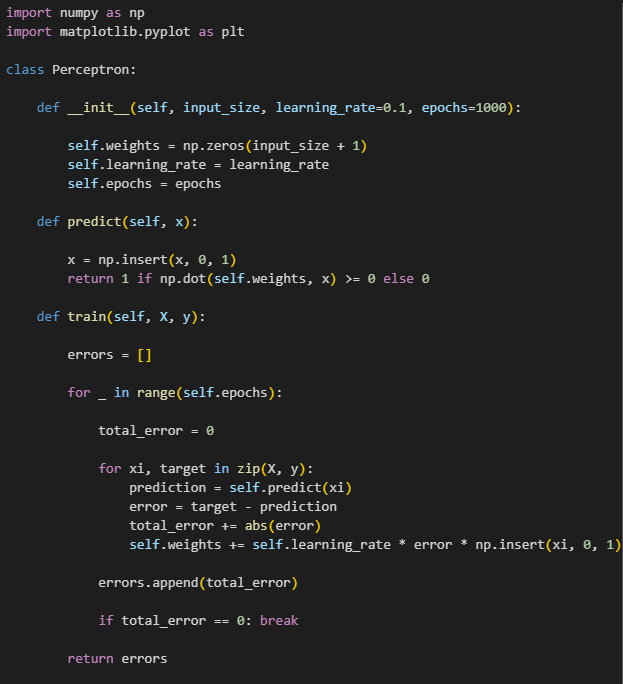
\includegraphics[width=.8\textwidth]{image1.png}
\end{figure}

A função descrita inicialmente define os pesos como zeros e os ajusta durante o treinamento, com base no erro entre as previsões e os valores esperados. A função \texttt{predict} calcula a soma ponderada das entradas (incluindo o bias, representado por um valor 1 adicional às entradas) e retorna 1 se o resultado for maior ou igual a 0; caso contrário, retorna 0.

O método \texttt{train} percorre os dados de entrada (\texttt{X}) e as saídas esperadas (\texttt{y}) durante um número predefinido de épocas. Durante esse processo, os pesos são ajustados proporcionalmente ao erro e à taxa de aprendizado. O treinamento para quando o erro total em uma época chega a zero. Além disso, os erros de cada época são armazenados para posterior análise e visualização do progresso do aprendizado.

\subsection*{Visualização do limite de decisão}

\begin{figure}[h]
	\centering
	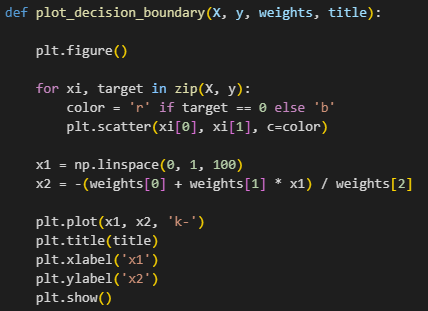
\includegraphics[width=.8\textwidth]{image2.png}
\end{figure}

A função implementada também permite plotar o limite de decisão.

\subsection*{Testando as portas com 2 inputs}

\begin{figure}[ht]
	\centering
	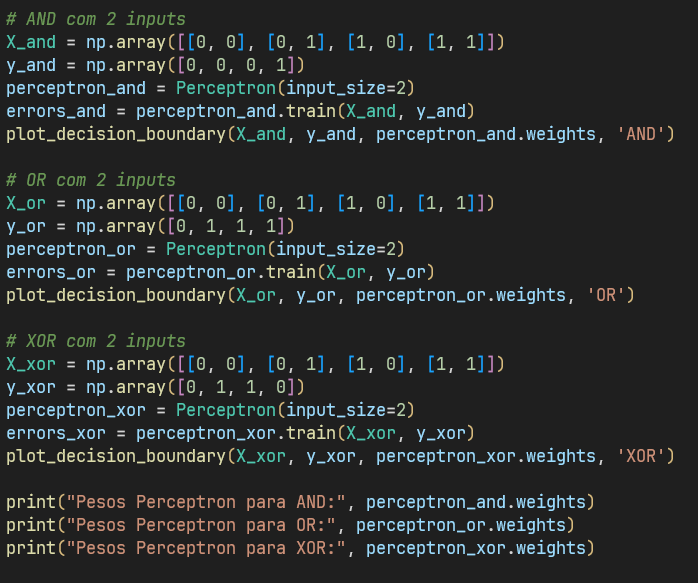
\includegraphics[width=.8\textwidth]{image3.png}
\end{figure}

\begin{figure}[ht]
	\centering
	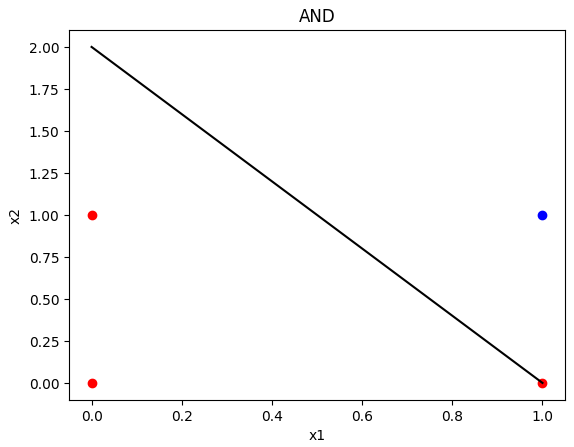
\includegraphics[width=.8\textwidth]{image4.png}
\end{figure}

\begin{figure}[ht]
	\centering
	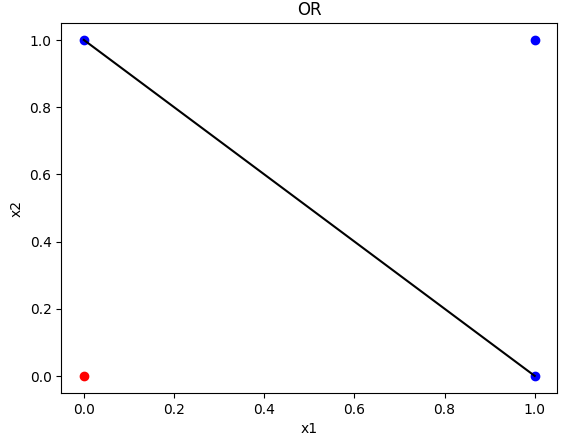
\includegraphics[width=.8\textwidth]{image5.png}
\end{figure}

\begin{figure}[ht]
	\centering
	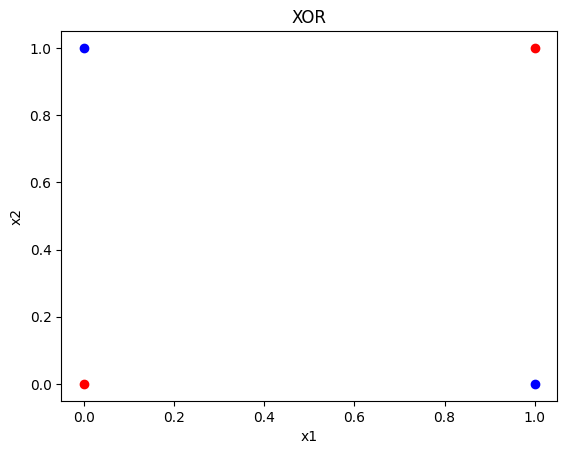
\includegraphics[width=.8\textwidth]{image6.png}
\end{figure}

Ao aplicar o perceptron na porta XOR, observa-se que ele não consegue separar os limites de cada grupo. Isso ocorre porque o perceptron é incapaz de lidar com problemas não linearmente separáveis, como demonstrado no gráfico.

\section*{Questão 2}

\begin{figure}[h]
	\centering
	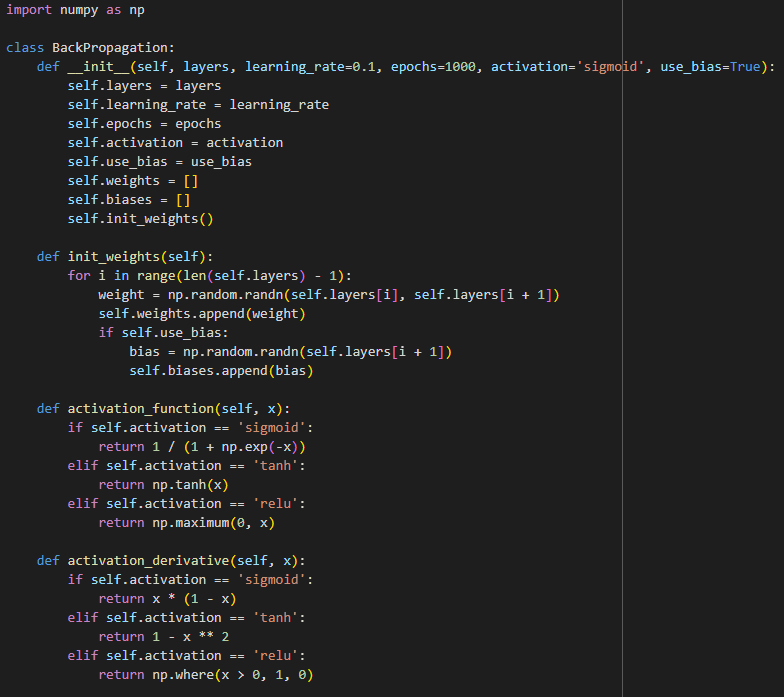
\includegraphics[width=.8\textwidth]{image7.png}
\end{figure}

\begin{figure}[h]
	\centering
	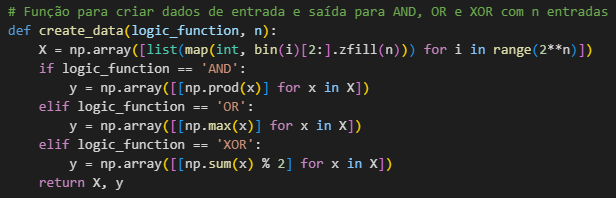
\includegraphics[width=.8\textwidth]{image8.png}
\end{figure}

\begin{figure}[h]
	\centering
	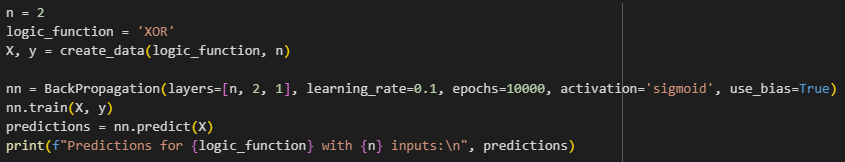
\includegraphics[width=.8\textwidth]{image9.png}
\end{figure}

\begin{enumerate}

	\item \textbf{A importância da taxa de aprendizado} \\
		A taxa de aprendizado determina o quanto os pesos e o bias são ajustados em cada iteração durante o treinamento. Um valor moderado é ideal, pois equilibra eficiência no aprendizado e estabilidade no processo. Métodos adaptativos, como Adam, podem melhorar significativamente o desempenho.

	\item \textbf{A importância do bias} \\
		O bias adiciona um deslocamento ao somatório ponderado das entradas, permitindo à rede aprender funções que não passam pela origem. Isso aumenta a flexibilidade e a capacidade de modelar funções complexas, sendo essencial em problemas práticos.

	\item \textbf{Funções de ativação e a relevância de suas derivadas} \\
		Funções de ativação aplicam transformações não lineares às saídas dos neurônios, permitindo que a rede modele relações complexas. A derivada da função de ativação é usada no \textit{backpropagation} para calcular os gradientes e ajustar os pesos.

		\begin{itemize}
			\item \textbf{Sigmoid:} Sofre de \textit{vanishing gradient} em redes profundas, mas é útil para saídas entre 0 e 1.
			\item \textbf{Tanh:} Melhora o aprendizado ao centralizar os valores em torno de 0, sendo uma alternativa superior ao Sigmoid.
			\item \textbf{ReLU:} Funciona bem em redes profundas, mas pode apresentar o problema de "neurônios mortos" (gradiente zero).
		\end{itemize}

		A derivada controla o ajuste dos pesos. Derivadas muito pequenas (como no Sigmoid em valores extremos) podem levar ao \textit{vanishing gradient}, dificultando o aprendizado. Por isso, funções como ReLU são mais robustas.

	\item \textbf{Por que o \textit{backpropagation} usa funções de ativação não lineares?} \\
		Sem funções não lineares, a composição de várias camadas resultaria apenas em transformações lineares. Isso limitaria a rede a resolver problemas linearmente separáveis, como o Perceptron. A introdução de não linearidade permite modelar relações complexas, como o XOR, expandindo significativamente o potencial de aprendizado da rede.
\end{enumerate}

\noindent \textbf{Código:} O código completo está disponível no \href{https://colab.research.google.com/drive/1TYKmfnGl8PGT1hnLn21a9-bw0shOEvjm?usp=sharing}{Google Colab}.

\end{document}
